\documentclass{beamer}

\usetheme{Madrid}

% Color settings
\setbeamercolor{normal text}{bg=white, fg=black}
\setbeamercolor{alerted text}{bg=white, fg=black}
\setbeamercolor{structure}{bg=white, fg=cyan!70}
\setbeamercolor{navigation symbols}{bg=white, fg=gray!50}
\setbeamercolor{title}{bg=cyan!7, fg=black}
\setbeamercolor{subtitle}{bg=white, fg=black}
\setbeamercolor{section in toc}{bg=white, fg=black}
\setbeamercolor{subsection in toc}{bg=white, fg=black}
\setbeamercolor{frametitle}{bg=cyan!7, fg=black}
\setbeamercolor{block title}{bg=white, fg=black}
\setbeamercolor{block title alerted}{bg=white, fg=black}
\setbeamercolor{block title example}{bg=white, fg=black}
\setbeamercolor{section number projected}{bg=white, fg=black}

% Header/Footer colors
\setbeamercolor{author in head/foot}{bg=cyan!7,fg=black} 
\setbeamercolor{title in head/foot}{bg=cyan!7,fg=black} 
\setbeamercolor{date in head/foot}{bg=cyan!7,fg=black} 
\setbeamercolor{page number in head/foot}{bg=cyan!7,fg=black}

% Redefine section in toc to include section numbers
\setbeamertemplate{section in toc}{\inserttocsectionnumber.~\inserttocsection}
%\setbeamertemplate{frametitle}[default][center]

\usepackage{graphicx} % for including graphics

\title[Construction Union\ldots{Historical-Comparative}]{Construction Union Agreements\\
Union Organizing in Historical-Comparative Perspective}
\author{Matthew Carson}
\date[Undergrad. Research Week '24]{Undergraduate Research Week 2024}

\begin{document}

\begin{frame}
  \titlepage
\end{frame}

\begin{frame}{Table of Contents}
  \tableofcontents
\end{frame}

\section{Argument}
\begin{frame}{Argument}
	US Building Trade unions organize their workers differently. Most labor unions compel employers to negotiate, but the Building Trades engage in voluntary negotiations, relying on workers' skill levels rather than strike leverage. 
	\newline\newline
	\textbf{Building Trades}
	\begin{itemize}
		\item Are frequently political outliers.
		\item Oppose progressive environmental policies.
		\begin{itemize}
			\item Alignin more closely with the petrochemical industry (e.g., pipelines).
		\end{itemize}
		\item Are not supportive of single-payer healthcare.
	\end{itemize}
	
	%This approach correlates with their frequent political deviations from the broader US labor movement, particularly in opposing progressive environmental policies and aligning more closely with the petrochemical industry on environmental issues, and not supporting single-payer healthcare.
\end{frame}


\section{Methods}
\begin{frame}{Methods}
\setlength{\arrayrulewidth}{0.0pt} % Set the thickness of the rules to 0
\begin{tabular}{|p{0.3\textwidth}|p{0.6\textwidth}|}
\hline
\begin{minipage}[t][0.2\textheight][t]{\linewidth}
Historical\\
Within-Case\\
Analyses
\end{minipage}
&
\begin{itemize}
    \item Historical trajectory of the union.
    \item Durability: institutional arrangements.
    \item Structural features \& constraints.
    \item Institutional changes (mergers, etc.).
    \item Evolutionary or generative approach.\footnote{Reed 1997}
\end{itemize}
\\
\hline
\begin{minipage}[c][0.2\textheight][b]{\linewidth}
Comparative\\
Between-Case\\
Analyses
\end{minipage}
&
\begin{itemize}
    \item Differences in institutional features.
    \item Difference in political outcomes.
\end{itemize}
\\
\hline
\end{tabular}
\end{frame}

\section{Union Organizing Paths}
\subsection{NLRB Election}
\begin{frame}{Union Organizing Paths: NLRB Election}
  \begin{columns}
    \column{0.725\textwidth}
    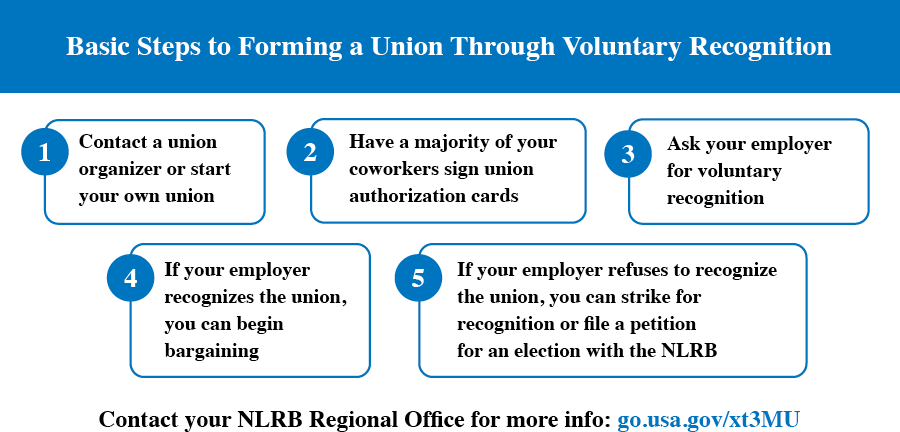
\includegraphics[width=0.9\linewidth]{../images/DOL}
    \begin{scriptsize}
	    \begin{center}
	    	(Source: US Department of Labor.)
	    \end{center}    
    \end{scriptsize}
    
    
    \column{0.275\textwidth}
     Designed for the \underline{industrial unions} forming at the time of the passage of the National Labor Relations Act.
    \newline\newline
    However, it was not designed for the Building Trades because they were already organizing differently.

    \end{columns}
\end{frame}

\subsection{Comparison}
\begin{frame}{Union Organizing Paths: Comparison}
  \begin{columns}
    \column{0.725\textwidth}
    \includegraphics[width=0.9\linewidth]{../images/organizing_paths}

    \column{0.275\textwidth}
    The industrial mode of organizing (left) and the construction mode of organizing (right).\newline\newline
    Construction unions may follow either path, but other unions may not voluntarily negotiate the way that construction unions can.
    \end{columns}
\end{frame}

\section{Union Leverage}
\begin{frame}{Union Leverage}
  \begin{columns}
    \column{0.725\textwidth}
    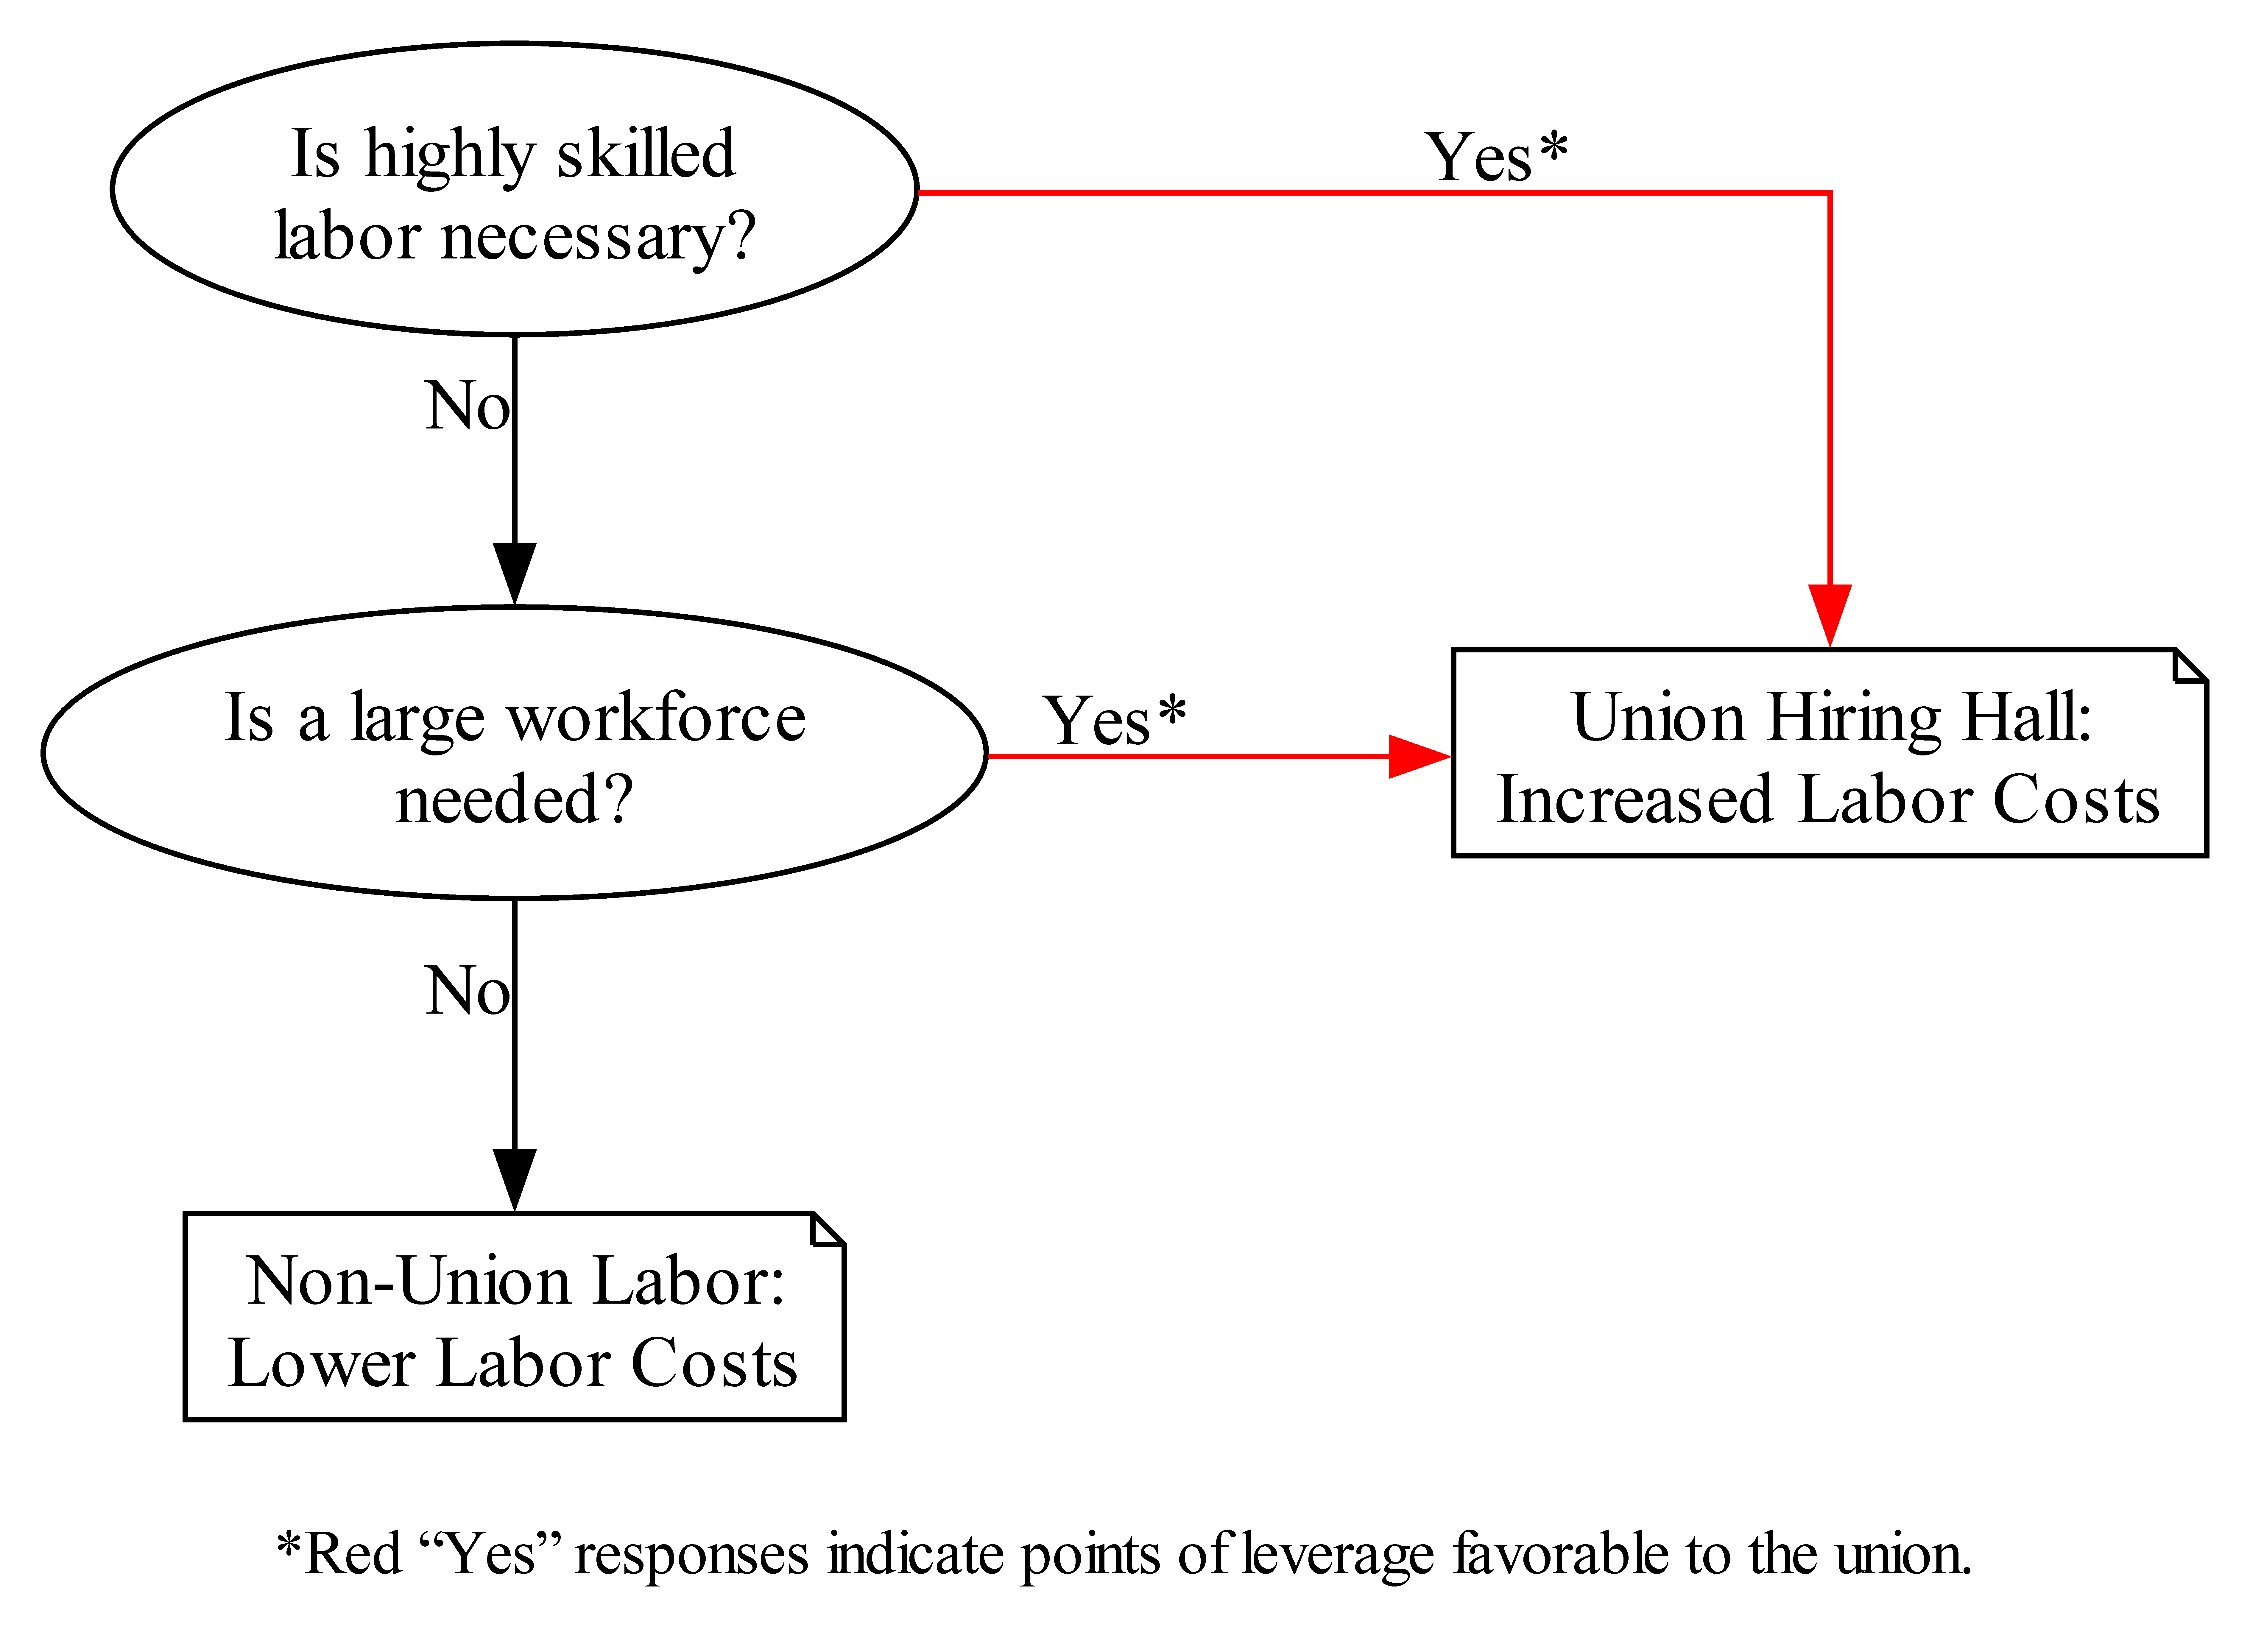
\includegraphics[width=\linewidth]{../images/union_power_red}

    \column{0.275\textwidth}
    Construction unions have more leverage where the employer requires a more skilled workforce or where the job is large and requires many employees.
  \end{columns}
\end{frame}

\section{Hiring Hall}
\begin{frame}{Hiring Hall}
	\begin{columns}
	\column{0.725\textwidth}
	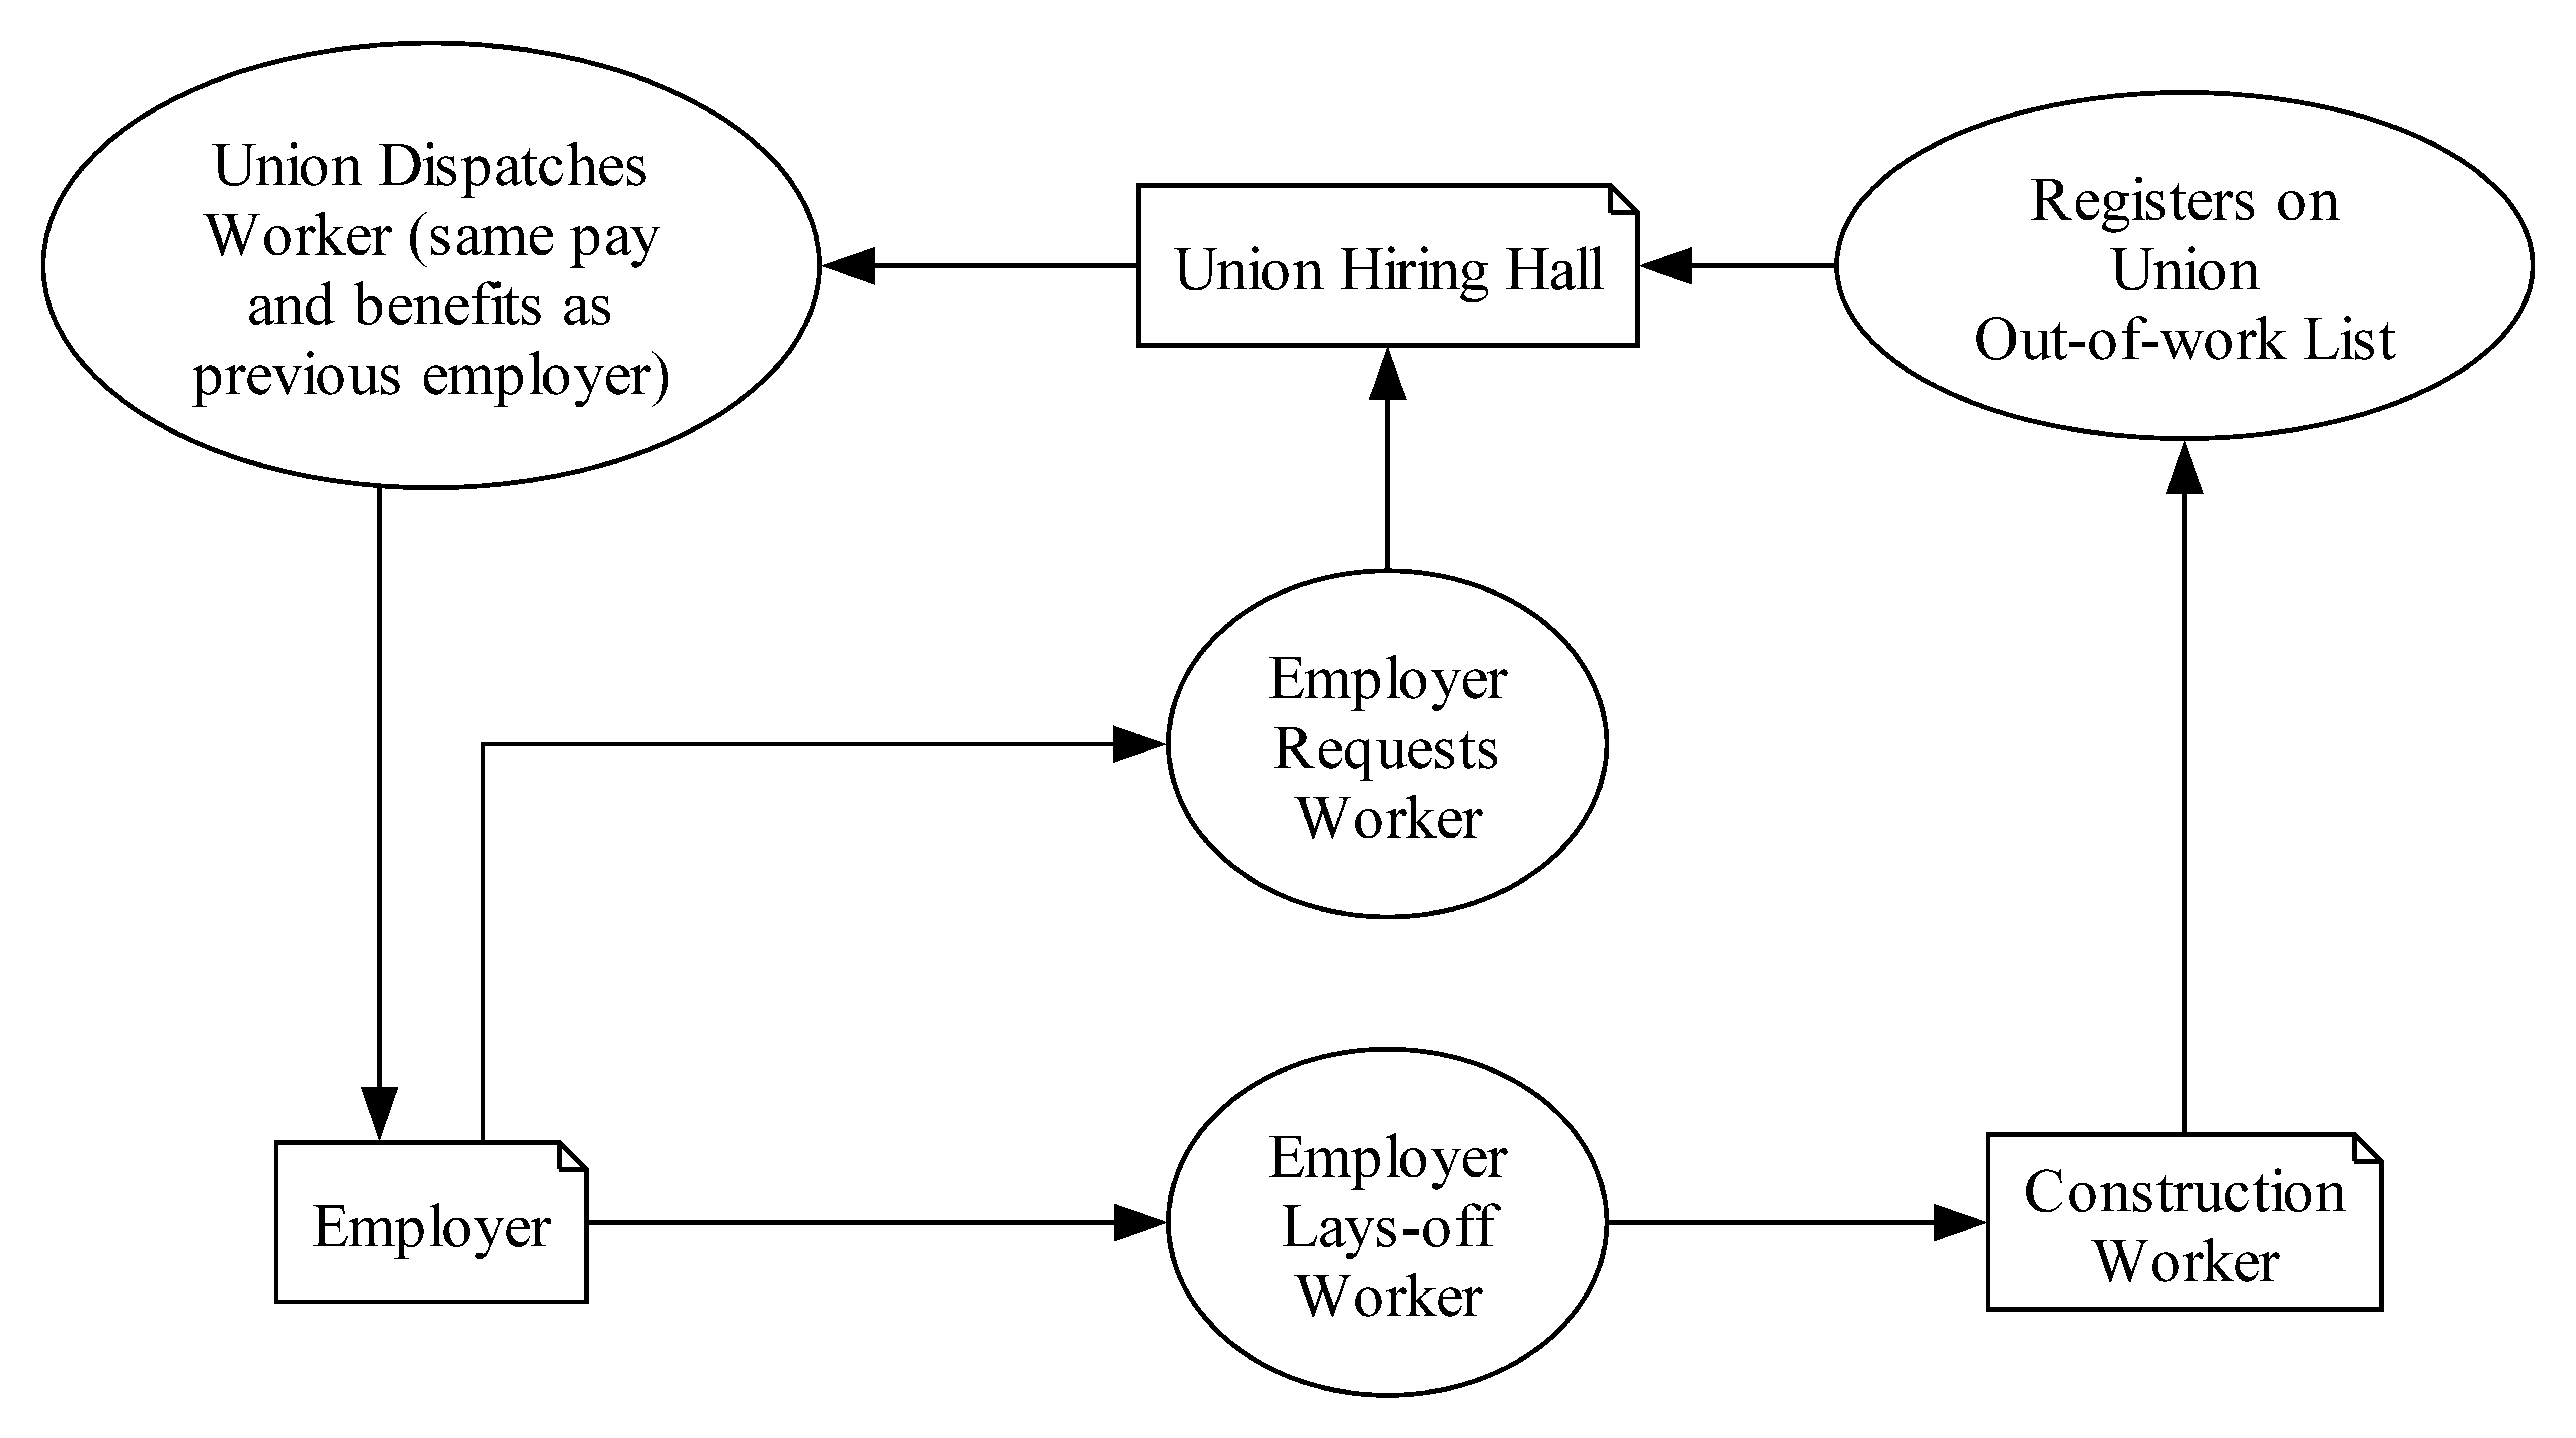
\includegraphics[width=\linewidth]{../images/hiring_hall}
	\column{0.275\textwidth}
	When employers require more workers for their projects, they contact the hiring hall to request workers to be dispatched to the job site.
	\end{columns}
\end{frame}

\section{Findings}
\subsection{Institutional consolidation}
\begin{frame}{Findings: Institutional consolidation}

	\begin{itemize}
		\item United Association (UA)
			\begin{itemize}
				\item Apprenticeship and training as a ``bargaining chip."
				\item Prehire agreements are the norm.
				\item Became a junior partner to capital because of institutional/structural. features.
	\end{itemize}
		\item OCAW/USW
		\begin{itemize}
			\item Never junior partner to capital -- relationship antagonistic
		\end{itemize}
	\end{itemize}
\end{frame}


\subsection{Different occupational context}
\begin{frame}{Findings: Different occupational context}
	\begin{itemize}
		\item United Association (UA)
		\begin{itemize}
			\item The pre-hire agreement made the movement between employers with the same wages/benefits possible.
			\item Hiring hall formed as an institution
		\end{itemize}
		\item OCAW/USW
			\begin{itemize}
				\item Same plant entire career
			\end{itemize}
	\end{itemize}
\end{frame}


\subsection{Political context}
\begin{frame}{Findings: Political context}
	\begin{itemize}
		\item United Association (UA)
		\begin{itemize}
			\item Never had Communist Party or socialist connections
		\end{itemize}
		\item OCAW/USW
			\begin{itemize}
				\item Historically had Communist Party members
			\end{itemize}
	\end{itemize}
\end{frame}

%		\item Different occupational context
%		\begin{itemize}
%			\item UA: contingent work
%			\begin{itemize}
%				\item The pre-hire agreement made the movement between employers with the same wages/benefits possible.
%				\item Hiring hall formed as an institution
%			\end{itemize}
%			\item USW: same plant entire career
%		\end{itemize}
%	\end{itemize}


\section{Conclusion}
\begin{frame}{Conclusion}
  This concludes my presentation.
\end{frame}

\end{document}
